
%
%  $Description: Author guidelines and sample document in LaTeX 2.09$ 
%
%  $Author: ienne $
%  $Date: 1995/09/15 15:20:59 $
%  $Revision: 1.4 $
%

\documentclass[times, 10pt,twocolumn]{article} 
\usepackage{latex8}
\usepackage{times}
\usepackage{graphicx}
\usepackage{epstopdf}
\usepackage{enumitem}
\usepackage[font=small]{caption}

%\documentstyle[times,art10,twocolumn,latex8]{article}

%------------------------------------------------------------------------- 
% take the % away on next line to produce the final camera-ready version 
\pagestyle{empty}

%------------------------------------------------------------------------- 
\begin{document}

\title{Distributed Software Transactional Memory}

\maketitle
\thispagestyle{empty}

\begin{abstract}

   The present paper describes the details of a distributed software
   transactional memory implementation.
   Solutions for 2 scenarios are presented: \\
   a) perfect links and processes \\
   b) fault-tolerant environment with replication \\
\end{abstract}



%------------------------------------------------------------------------- 
\Section{Introduction}
Due to the revolution in the computing world and marketing strategies, today’s world has moved to cloud based services rather than maintaining their own networks. The cloud service providers are well
equipped with the hardware and software infrastructure to provide better services because of the aspect of Distributed computing. 

In this model of computing one of the main problems that the providers has to face is the concurrent transactions. How the system behave when multiple users access the same object at the same 
time and manipulates them. How to maintain the proper order of commit and how to resolve conflicting manipulations. Here in this paper we are going to address this problem deeper and propose 
a solution which can be implemented and evaluated during next few weeks ahead.

In the following sections the implementation of a distributed software transactional memory library is presented for two scenarios: \\
a) perfect Master, Servers and links \\
b) perfect Master, links and recoverable, sequentially \\

Section \ref{sec:arch} introduces an overview of each scenario. Section 
\ref{sec:algor} discusses the algorithms used for concurrency control, 
transaction management and Client-Server communication


%------------------------------------------------------------------------- 
\Section{Architecture}
\label{sec:arch}

The assumption made for all the sections below is that the Master is a perfect process. The names Object Servers and Servers are used interchangeably and refer to any non-Master and non-Client process that participates in a transaction.
The main differences/similarities between the two architectures, perfect and fault-tolerant, are the following:
\begin{itemize}[noitemsep,nolistsep]
\item for perfect, the Coordinator of a transaction can be any Server, not necessarily the Master
\item in the fault-tolerant scenario, replication of tentative objects and transactions is assured
\item the Master also acts as a failure detector in both scenarios 
\item the Master and the Coordinator are the same process in the fault-tolerant scenario
\end{itemize}

Subsection \ref{subsec:perf} details the perfect architecture, while Subsection \ref{subsec:ftsys} lists the details of the fault-tolerant architecture. Further details on the reponsibilities of the Coordinator/Master are in Subsection \ref{subsec:respon}.
%------------------------------------------------------------------------- 
\SubSection{Perfect links and processes}
\label{subsec:perf}
As illustrated in Figure \ref{fig:perf}, the Master server {\it(M)} is used by the Object Servers {\it(S)} when bootstrapping. Information such as
IP address and port number of the Server is stored by the Master which, then, issues unique identifiers for each Server. Once the Object Server (S) has been issued an identifier and notified the Master of joining the group of available servers, it can be connected by Clients {\it(C)} for handling transactions. Transaction identifiers (TID) should be unique to the whole system therefore the Master server (M) will keep track of the global sequence of TIDs.

\begin{figure}
\centering
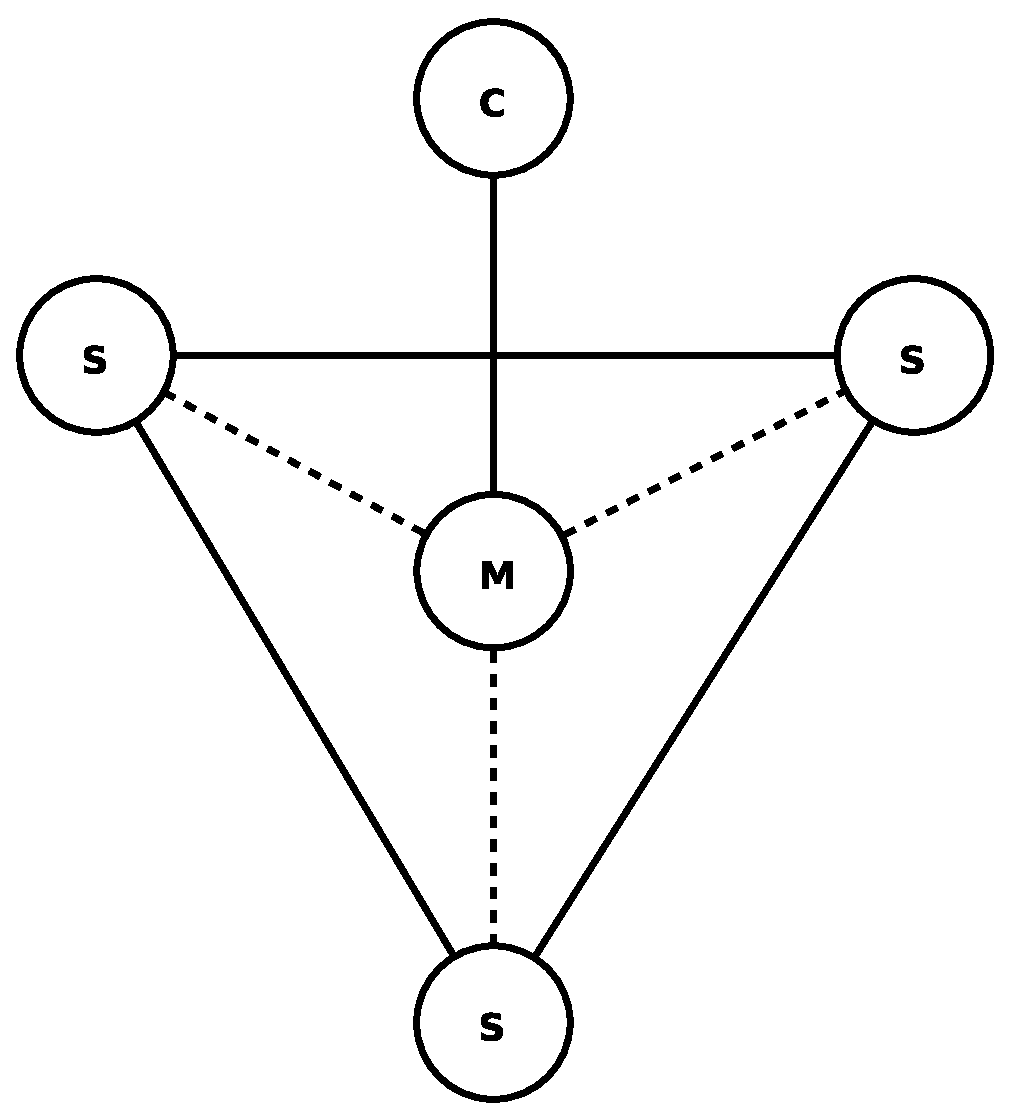
\includegraphics[scale=0.3]{perfect.eps}
\caption{Master, Server and Client entities in a perfect setup}
\label{fig:perf}
\end{figure}

Note: the number of Object Servers can vary.

Clients (C) will query the Master (M) if the their cached list of servers is outdated or attempting to reach an Object Server (S) times out. The Master (M) provides the Client an updated list of the available Object Servers (S) to be used for establishing/handling transactions.

Objects that are going to be stored in Object Servers (S) have unique identifiers (integer) so that each object can be uniquely identified throughout the system. Therefore in this solution we are using the modulo function against the number of Object Servers (S) available in order to find the actual location of the object to be stored or referred.

The clients (C) can connect to multiple Object Servers inside a single transaction, hence it is required to have a Coordinator that manages the transaction operations such as commit and abort.
The Coordinator can be any Server from the list provided by the Master in the current, perfect, scenario. On the other hand, in the fault-tolerant scenario, we consider the Master (M) as the coordinator. When a Client (C) needs to manipulate an object it connect to the relevant Object Server, which will contact the Coordinator (M) and join the transaction. Then the manipulation operations (Read/Write) are handled only by the Client and the Object Servers (S).

%------------------------------------------------------------------------- 
\SubSection{Fault Tolerant system}
\label{subsec:ftsys}
For recoverability in case of failure, an extension to the above system is necessary. Having a replication of the transaction's objects in a particular Object Server (S) across other Servers (S) is necessary to assure recoverability. The Master (M) handles the replica location of each Server. Our proposal for the replica locations is a conceptual ring, where S1's replica is stored in S2, and that of S2 in S3, etc. The Master notifies each Server of its replica location. The transaction modal is similar to the phase one, the only extension required is to ask the replica server as well to join the coordinator for the transaction.

The Master server (M) also assumes the role of a {\it failure detector}, by using the heartbeat messages regularly exchanged between the Master and the Server. In case of an Object Server(S) failure, the Master server(M) will identify it through heartbeats and issue a notification to all the other Object Servers (S) about the failure. No further TIDs are issued for the clients until the failure recovered. Once the current transactions complete, the Master will stabilise the system with the correct replica locations.

At the fault recovery, the Master server (M) will issue a notification to the Object Servers (S) asking to rearrange, so that the Object Servers (S) go through the list of objects which it is responsible and apply the modulo function again according to the new Object server count. All the Object Servers (S) process this action simultaneously and the object movement among servers will stabilize the system. Once the system is stable, the Master (M) will issue another notification to the Object Servers to invalidate the current replica object set and replicate the new object set. After this replication step the system becomes stable and the Master Server (M) starts to issue TIDs again. Furthermore, if a new server is added to the system, exactly the same steps mentioned above will be followed by the system.

%------------------------------------------------------------------------- 
\SubSection{Coordinator/Master responsiblities}
\label{subsec:respon}

The Coordinator's responsabilities and interface are different for the two scenarios (perfect and fault-tolerant) detailed in Section \ref{sec:arch}. For instance, assuming perfect links and processes, the Coordinator can be any of the Servers, thus reducing the Master's load. The list of servers available to the Client is supplied by the Master and it's updated with every server group membership change.

The Coordinator's responsibilities below are shared in both scenarios:
\begin{itemize}[noitemsep,nolistsep]
\item assign a transaction identifier to the Client 
\item handle abort and commit commands from the Client or Object Servers 
\item interface with the participant servers in the transaction during the voting and commit phases 
\end{itemize}

The Master also assumes the role of a failure detectore through the use of heartbeat messages. In the fault-tolerant environment, the Master also assumes the Coordinator role.
%------------------------------------------------------------------------- 
\Section{Algorithms}
\label{sec:algor}
In the subsections below, algorithms for communication, concurrency, deadlock detection and transaction management are enlisted.

%------------------------------------------------------------------------ 
\SubSection{Communication}
The following communication occurs {\bf before} the Client attempts connection to the Master node - between the Master and the Servers.

\begin{enumerate}
\item Master boots, followed by the Object Servers bootstrapping
\item During Object Servers bootstrap:
\begin{itemize}[noitemsep, nolistsep]
\item Master identifies the Object Servers trying to connect
\item Master assigns a unique name to the Object Servers to later be used as a reference
\end{itemize}
\item Object Servers's heartbeat messages periodically being sent to Master. Heartbeats are also used for replica management in the faul-tolerant scenario. Should one of the replicas fail, the objects are replicated in another server in order to maintain a certain level of availability in the system.
\end{enumerate}

Upon {\it attempting a transaction} the following communication exists between the Client, Master and Object Servers in a {\bf fault-tolerant} environment: 
\begin{enumerate}
\item Client connects to the Master and requests a transaction identifier 
\item Master maintains a global transaction sequence and returns a unique transaction identifier (TID) to the Client. Furthermore, a list of healthy Object Servers is also returned to the Client. 
\item Client generates a unique ID (integer) when generating the object and also be used in order to select an available server from the list (used in a modulo function)
\item Client uses the modulo result to connect to the Object Server and store the object representing the tentative versions of the transaction.
\end{enumerate}

The main difference between the above steps and the communication in a {\bf perfect} environment is that the TID is not necessarily assigned by the Master, but any of the Servers.

When the Client attempts to {\bf manipulate an existing object} in the {\it perfect} environment, the following communication takes place:
\begin{enumerate}
\item Client requests and retrieves TID from Master
\item Client retrieves object's previously generated unique ID
\item Client applies modulo on the retrieved ID to locate the relevant Object Server to request for reference
\item With the retrieved object reference, client can manipulate the object value
\end{enumerate}

%------------------------------------------------------------------------- 
\SubSection{Transaction Management and Concurrency Control}
\label{subsec:transmgt}
The {\it Flat Transaction} model allows for a client to manipulate objects on multiple servers in a single transaction. With regards to concurrency control, {\it Timestamp Ordering} will be used for this project. Figure \ref{fig:flat} illustrates a flat transaction model setup with a transaction being executed from the client on 3 servers.

\begin{figure}
\centering
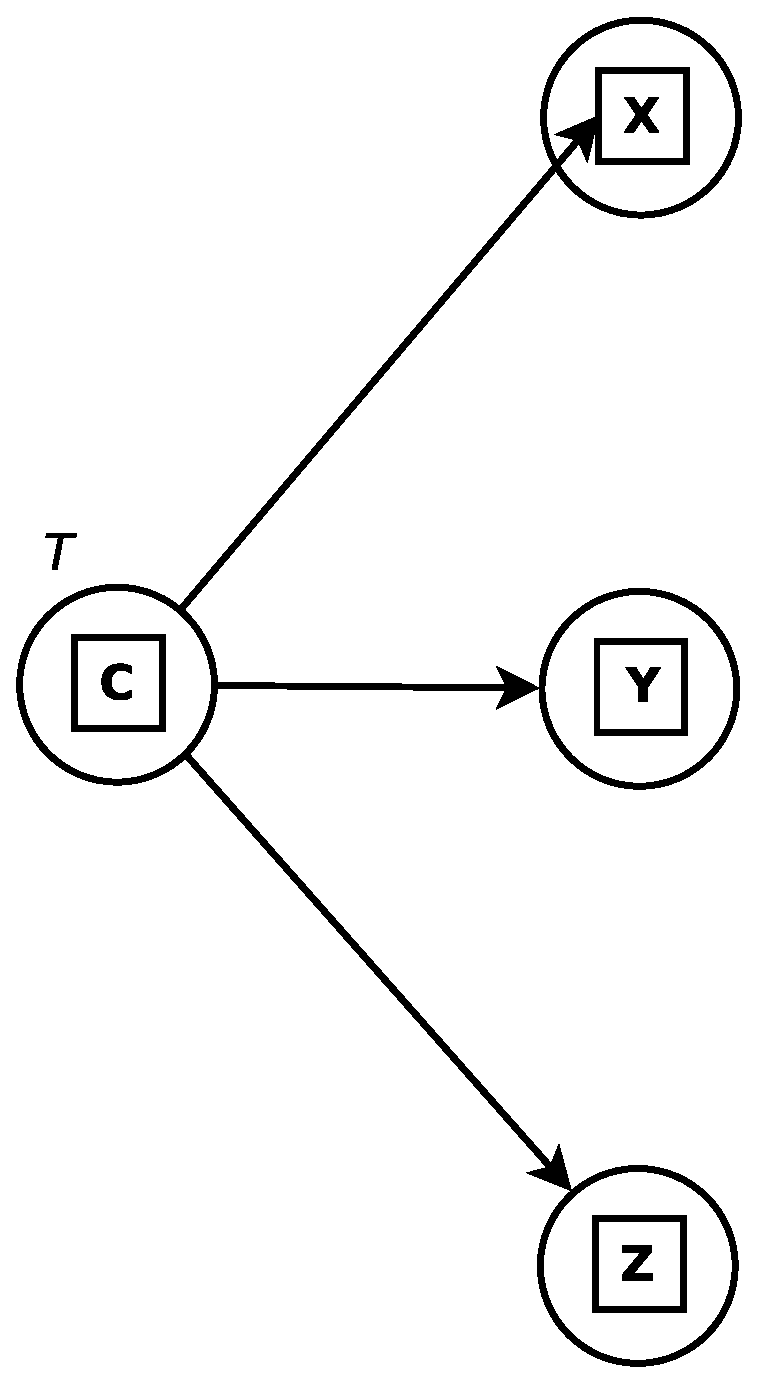
\includegraphics[scale=0.2]{flat-transaction.eps}
\caption{Flat Transaction model between a Client and 3 Servers}
\label{fig:flat}
\end{figure}


The advantages of choosing {\it Timestamp Ordering} over {\it Two-Phase Locking} or {\it Optimistic Concurrency} options are the following: 
\begin{itemize}[noitemsep, nolistsep]
\item Deadlock prevention - common with the use of locks
\item Better performance for transactions with predominantly {\it read} operations \cite{bernstein1987concurrency}
\item Faster conflict resolution when compared to locking - transactions are aborted immediately.
\end{itemize}

Figure \ref{fig:transa} illustrates the steps between the Client, Coordinator, Master and Object Serves during a transaction. The steps below offer more details on the communication that occurs in a perfect setup: 

\begin{itemize}[noitemsep, nolistsep]
\item {\bf Steps 3-4:} Client acquires transaction ID from the Coordinator 
\item {\bf Step 5:} Client passes TID to the Object Server
\item {\bf Step 6:} Object Server calls the Coordinator's {\it inteface}
\item {\bf Steps 7-8:} Client manipulates objects directly on the Object Server
\item {\bf Step 9:} Upon transaction end, Client asks the Coordinator to either {\it Abort} or {\it Commit} 
\item {\bf Step 10:} Coordinator will request each participant server in the transaction to indicate whether it can commit a transaction or not.{\it (Voting Phase)}
\item {\bf Step 12:} If all participants answer/vote {\it positively}, the Coordinator issues {\it doCommit(TID)} for each parcipant to commit its part of the transaction
\item {\bf Step 13:} Once completed, all servers acknowledge the commit and Coordinator notifies the Client that it's successful -{\bf Step 14}
\item Should any of the participant servers be unable or disagree to commit and aborts, the Coordinator will request all the remaining participants to abort. Client will then be notified.
\end{itemize}

\begin{figure}
\centering
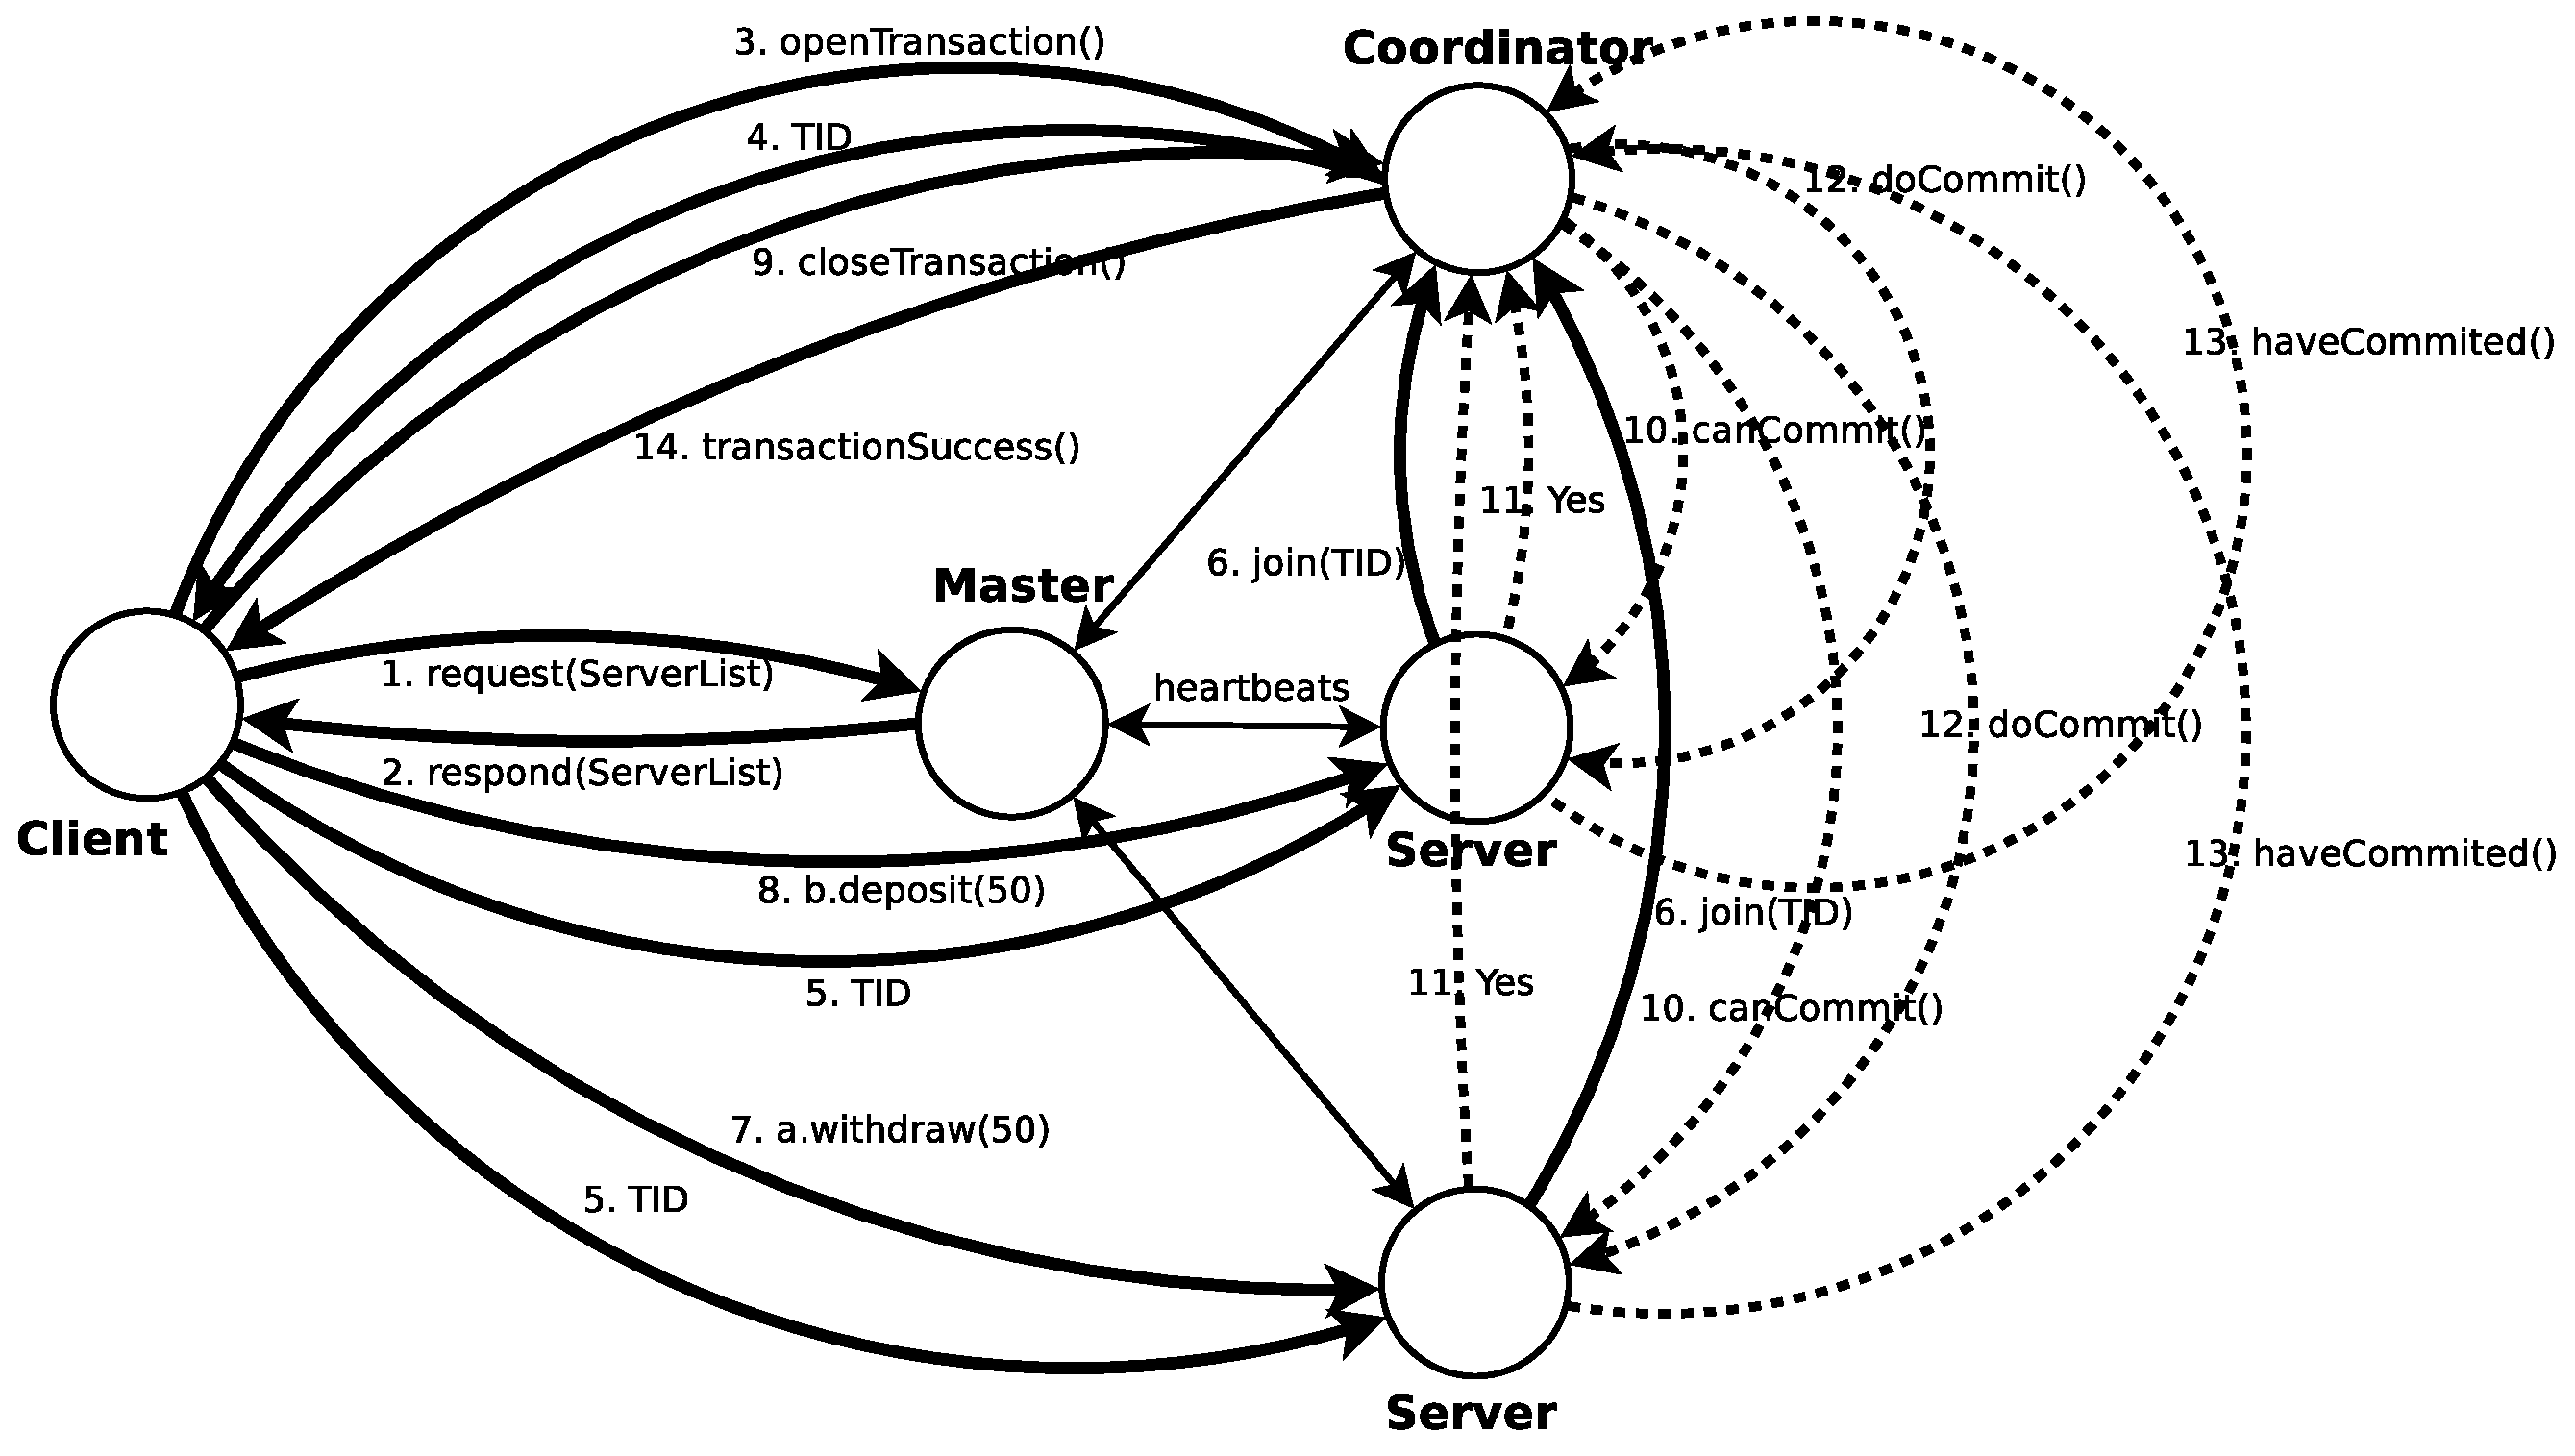
\includegraphics[scale=0.2]{transaction.eps}
\caption{Transaction steps between the Client, Master, Coordinator and Servers. The dotted lines represent the 2-phase distributed commit}
\label{fig:transa}
\end{figure}



%-------------------------------------------------------------------------
\SubSection{Timestamp Ordering and Deadlock Detection}
\label{subsec:dldetect}
Due to the use of timestamp ordering for concurrency control, there is limited probability of deadlock occurance.
Each transaction is assigned a unique timestamp on start. Each operation in a transaction is validated when it is carried out.
Should a transaction fail the validation it is immediately aborted, but can be restarted by the Client. The Client is issued with a globally unique transaction timestamp by the Coordinator. The servers are jointly responsible for ensuring serial equivalence. For instance, server S1 access an object before S2, thus server S1 appears before S2 for all objects. The Coordinators must agree on timestamp ordering to maintain all servers synchronised with the same ordering. The timestamp consists of a {\it (local timestamp, server-id)} pair and is kept synchronized by the use of local physical clocks coordinated by the Master.

Conflict resolution is performed at each operation.
The basic timestamp ordering rule is based on operation conflicts and is very simple:
{\it A transaction’s request to write an object is valid only if that object was last read and written by earlier transactions. A transaction’s request to read an object is valid only if that object was
last written by an earlier transaction.}\cite{coulouris2005distributed}. Each transaction has its own tentative version of each object it accesses, such that multiple concurrent transactions can access the same object. The tentative versions of each object are committed in the order determined by the timestamps of their transactions by transactions waiting, if necessary, for earlier transactions to complete their writes.
Since transactions only wait for earlier ones (thus, no cycle occurs in the wait-for graph), no deadlocks occur.

Conflict resolution is performed at each operation. If the resolution is to abort the transaction the Coordinator is informed and it will abort the transaction for all the participants.

%--------------------------------------------------------------------------
\SubSection{Replication}
\label{subsec:faultol}
The fault tolerant design supports failure of a single Object Server. It extends the perfect architecture by assuring the replication of objects in the adjacent server.
For instance, the object stored in Object Server S1 keeps a copy in S2 as a replica. The Master server is responsible for keeping track of the replica servers.

When an Object Server {\bf fails}:
\begin{enumerate}[noitemsep, nolistsep]
\item Master detects the failure from the absence of heartbeat messages from the server
\item Master server issues a {\it “failure warning notification”} to the other servers, so that the current transactions related to the absent server be aborted.
Others will continue but new transactions will not be accepted. (Master no longer issuing TIDs)
\item Master coordinates the object replication so that the currently available servers share the objects held by the absent server.
\item Once the Master notifies all the servers about the new, stable status, transactions can be take place again.\\
\end{enumerate}

When the failed server {\bf recovers}:
\begin{enumerate}[noitemsep, nolistsep]
\item Master detects the arrival of a new server
\item Master server issues a {\it “New server notification”} for the servers. Once the current pending transactions are completed, servers are stabilized
\item Master server coordinates object replication such that a portion of objects in the current system will be transferred to the new server
\item Once the Master notifies all servers of the stabilized status, transactions can be resumed
\end{enumerate}

%------------------------------------------------------------------------- 
\Section{Conclusion}
Across the sections we discussed the solutions proposed in order to implement Distributed Software Transactional Memory System.
Our solution addresses two scenarios: perfect links and processes and a fault tolerant system.
A very important goal has been to provide a simple solution which would eliminate conflicts in transactions without encountering the inefficiency of a distributed environment. 
The sections and subsections address each of the two architectures individually in order to provided a clearer distinction of responsibilities and complexity of the system.
Furthermore,{\it Timestamp Ordering} based concurrency control aids in eliminating local and global deadlocks which represents one of the major issues that need to be addressed in DSTMs.

Finally, we believe that the concepts we came across in the discussion of this paper builds a firm foundation for implementing this solution in an efficient manner.
%------------------------------------------------------------------------- 
%- \Section{References}

\bibliographystyle{latex8}
\bibliography{latex8}

%------------------------------------------------------------------------- 
\end{document}

